
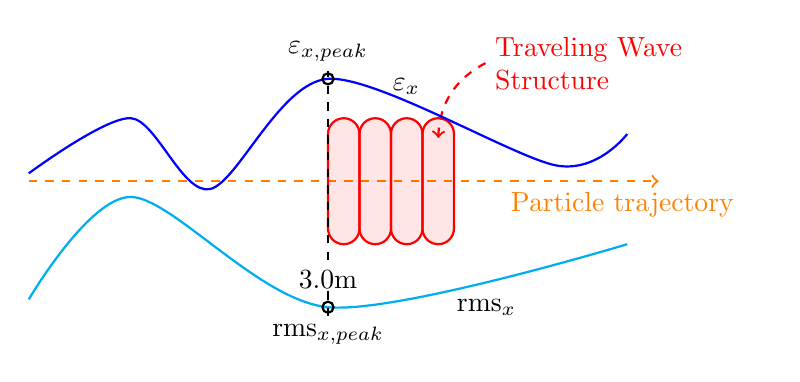
\begin{tikzpicture}

  \draw[dashed, thick, color=orange] (1.2,2.0) edge[->] (9.2,2);
  \node[orange, right, text width=3.2cm] at (7.2, 1.7) {Particle trajectory};

  %\draw[thick] (1.2,2.5) edge (9,2.5);
  %\draw[thick] (1.2,1.5) edge (9,1.5);
  %\node[above] at (1.0, 1.45) {Beam pipe};

  \draw[thick,color=red, fill=red, fill opacity=0.1, rounded corners=2mm] (5.0,1.2)
      rectangle (5.4,2.8);
  \draw[thick, dashed] (5.0,1.0) edge (5.0,3.4) node[below] {$3.0$m};
  \draw[thick,color=red, fill=red, fill opacity=0.1, rounded corners=2mm] (5.4,1.2)
      rectangle (5.8,2.8);
  \draw[thick,color=red, fill=red, fill opacity=0.1, rounded corners=2mm] (5.8,1.2)
      rectangle (6.2,2.8);
  \draw[thick,color=red, fill=red, fill opacity=0.1, rounded corners=2mm] (6.2,1.2)
      rectangle (6.6,2.8);
  \node[right, red, text width=2.8cm] at (7.0, 3.5) {Traveling Wave Structure};
  \draw[dashed, thick, color=red, bend right] (7.0,3.5) edge[->] (6.4,2.55);

  \draw[thick, cyan] plot [smooth, tension=0.5] coordinates {
      (1.2,0.5)
      (2.5,1.8)
      (5.0,0.4)
      (8.8,1.2)};
  \draw[thick, dashed] (5.0,0.6) edge (5.0,0.2);
  \draw[thick] (5.0,0.4) circle (2pt);
  \node[very thick, right] at (6.5, 0.4) {rms$_x$};
  \node[below] at (5.0, 0.3) {rms$_{x\text{, peak}}$};

  \draw[thick, blue] plot [smooth, tension=0.5] coordinates {
      (1.2,2.1)
      (2.5,2.8)
      (3.5,1.9)
      (5.0,3.3)
      (7.9,2.2)
      (8.8,2.6)};
  \draw[thick] (5.0,3.3) circle (2pt);
  \node[right] at (5.7, 3.2) {$\varepsilon_x$};
  \node[above] at (5.0, 3.4) {$\varepsilon_{x\text{, peak}}$};

\end{tikzpicture}
